\chapter{FLOCKING ALGORITHM}

% introduction
\section{Introduction}
The behavior seen in social animals like birds and fishes is called \textit{flocking}. Flocking can be used to simulate this social behavior between entities by following a set of simple rules. These rules were introduced by the pioneer of flocking Craig Reynolds\cite{craig1}. The three main steering behaviors are: separation, alignment, and cohesion. In this chapter we are going to discuss the different behaviors implemented in our code, which include the three main steering behaviors, along with a few others.

% 3 steering behaviors
\section{Three Main Steering Behaviors}
These steering behaviors are velocity vectors, they have direction and magnitude. Each behavior is evaluated at each time step for each boid.

% separation
\subsection{Separation}
\textit{Separation} can be described as the steering force that would maintain each entity of the flock separated by at least a minimum determined distance. Craig Reynolds first called this rule \textit{collision avoidance} because he meant to avoid collision with nearby flockmates. Later on, the rule was named \textit{separation}. This steering behavior prevents crowding between the boids. As can be seen in Figure~\ref{separationPDF} we only consider the flockmates within a certain radius when we evaluate this behavior. The red vector is the obtained steering force with this behavior.

% separation figure
\begin{figure}[htbp]
\begin{center}
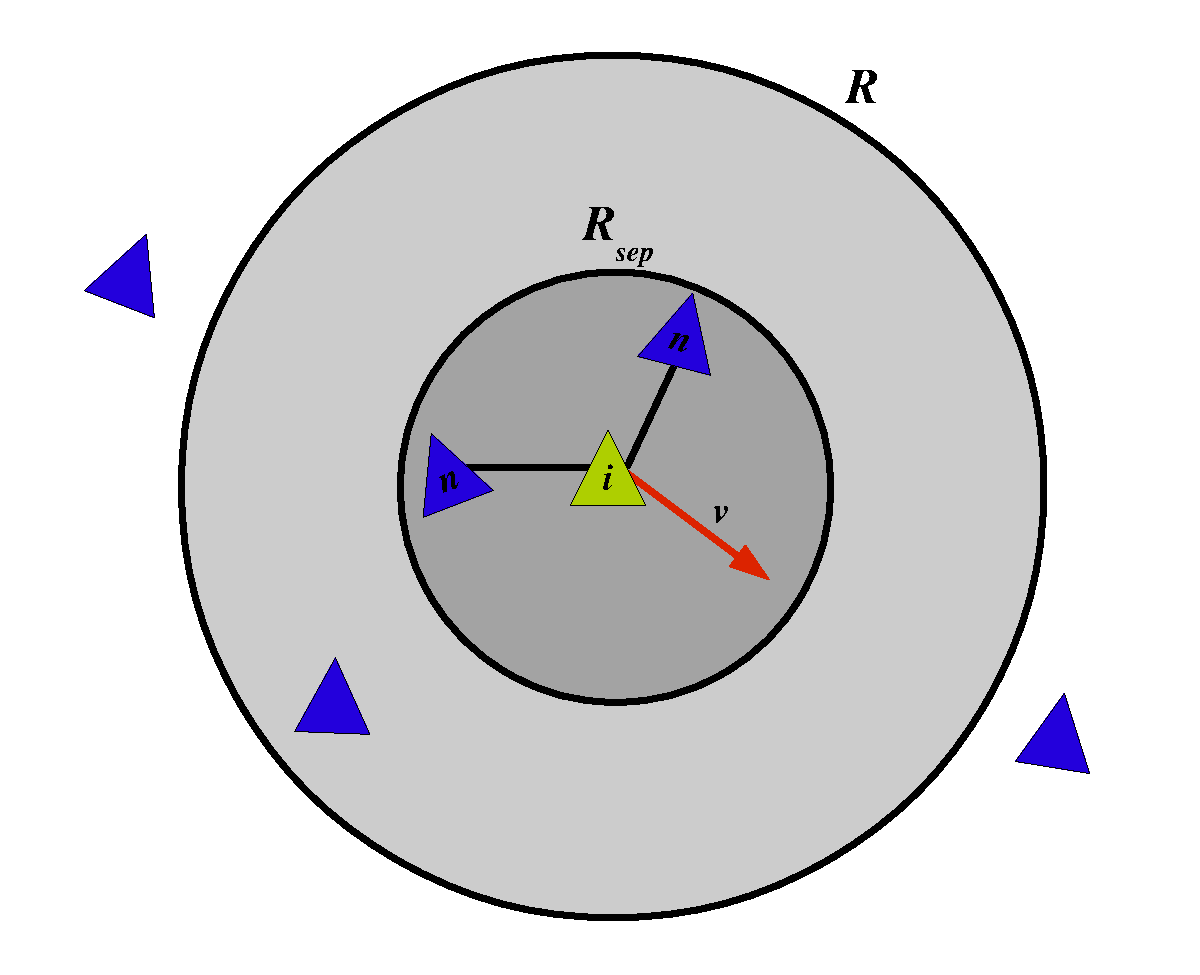
\includegraphics[scale=0.3]{figures/separation.pdf}
\caption{Separation steering force}
\label{separationPDF}
\end{center}
\end{figure}

We can said that separation is a repulsive force. The mathematical expression that we implemented is showed in equation~\ref{separationEquation}.

% separation equation
\begin{equation}
\label{separationEquation}
Separation =\frac{1}{M} \sum_{n=1}^{M} \frac{\overline{p_i - p_n}}{d(p_i,p_n)}
\end{equation}

Where $M$ is the number of boids within the minimum distance from the boid in question, $p_i$ is the position of boid $i$, and $d(p_i,p_n)$ is the distance between boids $i$ and boid $n$.

We first loop over the nearest neighbors, then for this rule we only pick the neighbors that are with the minimum separation distance, we sum up the normalization of difference between the positions of boid $i$ and boid $n$ divided by the distance of boid $i$ from boid $n$. Then, we average over the number of boids that were within the minimum distance to finally get the the vector that is going to correct the heading and speed of the \textit{separation} of boid $i$  and their nearest neighbors. 

% alignment
\subsection{Alignment}
\textit{Alignment} is the steering behavior that match the heading of all boids. Reynolds initially called this behavior \textit{velocity matching}, later the name was changed to \textit{alignment}. This behavior also prevents crowding along with \textit{separation}. As the name of the rule said, each boid would \textit{align} itself with the average velocity of the local neighborhood. Align with respect of direction and/or speed. Figure~\ref{alignmentPDF}  shows the corrective steering force vector in red.

% alignment figure
\begin{figure}[htbp]
\begin{center}
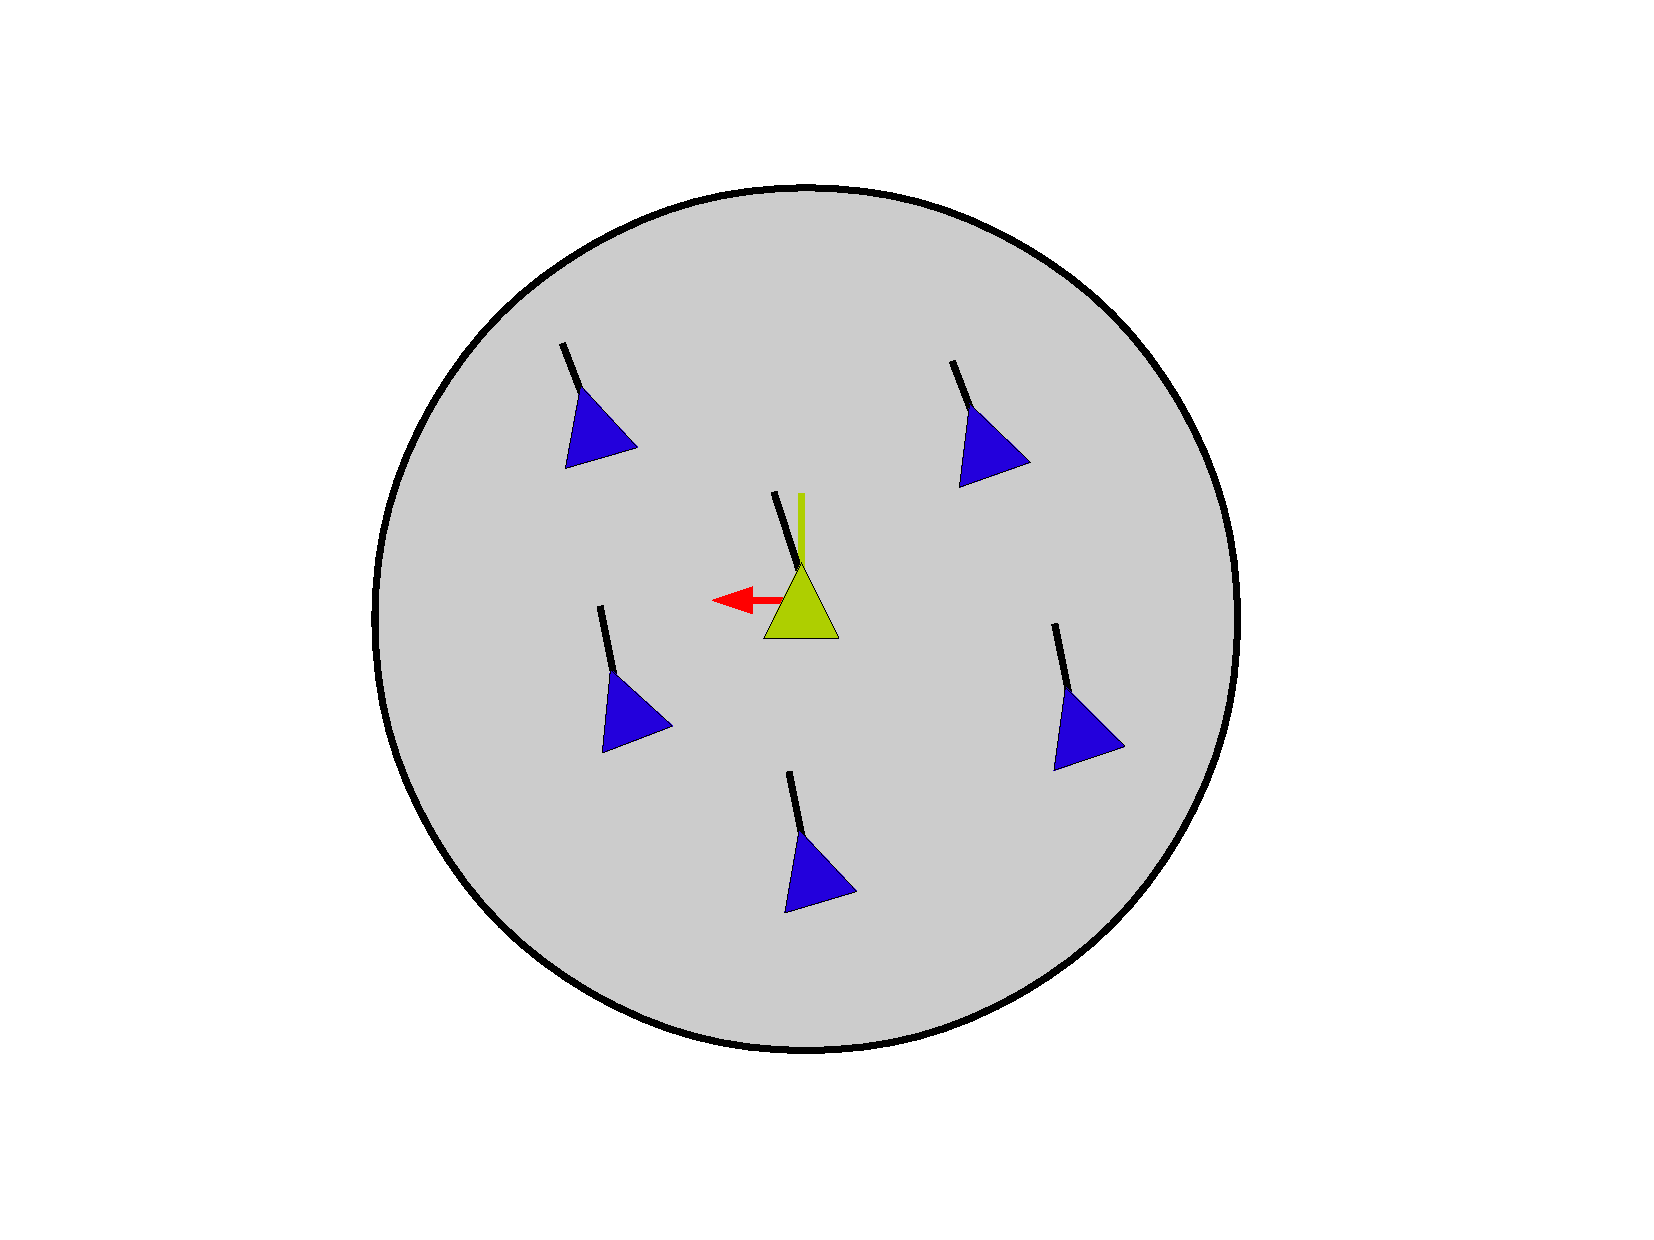
\includegraphics[scale=0.3]{figures/alignment.pdf}
\caption{Alignment steering force}
\label{alignmentPDF}
\end{center}
\end{figure}

\textit{Alignment} is also calculated in the local neighborhood of the boid in question. This steering behavior was computed using equation~\ref{alignmentEquation}.

% alignment equation
\begin{equation}
\label{alignmentEquation}
Alignment = \left[  \frac{1}{N} \sum_{n=1}^{N} v_n \right ] - v_i
\end{equation}

Where $N$ is the number of boids in the nearest neighbor within the search radius, this radius is bigger than the radius of the minimum separation distance used for \textit{separation}. $v_n$ is the velocity of boid $n$, we average the velocities of all boids inside the neighbor, then we subtract the velocity of the current boid from it to finally get the \textit{alignment} corrective force.

% cohesion
\subsection{Cohesion}
\textit{Cohesion} is the behavior that steers towards the center of the flock. When Reynolds introduced its \textit{Boids} model, he called this behavior \textit{flock centering} and defined as \textit{the attempt to stay close to nearby objects}. The definition was kept while the name of the rule changed to \textit{cohesion}. This behavior makes each boid attracted to the center of the flock, in our case we calculated it using the local neighbor of each boid, so they would be attracted to the center of their local neighbor.  Figure~\ref{cohesionPDF} shows the \textit{cohesion} steering force in red.

% cohesion figure
\begin{figure}[htbp]
\begin{center}
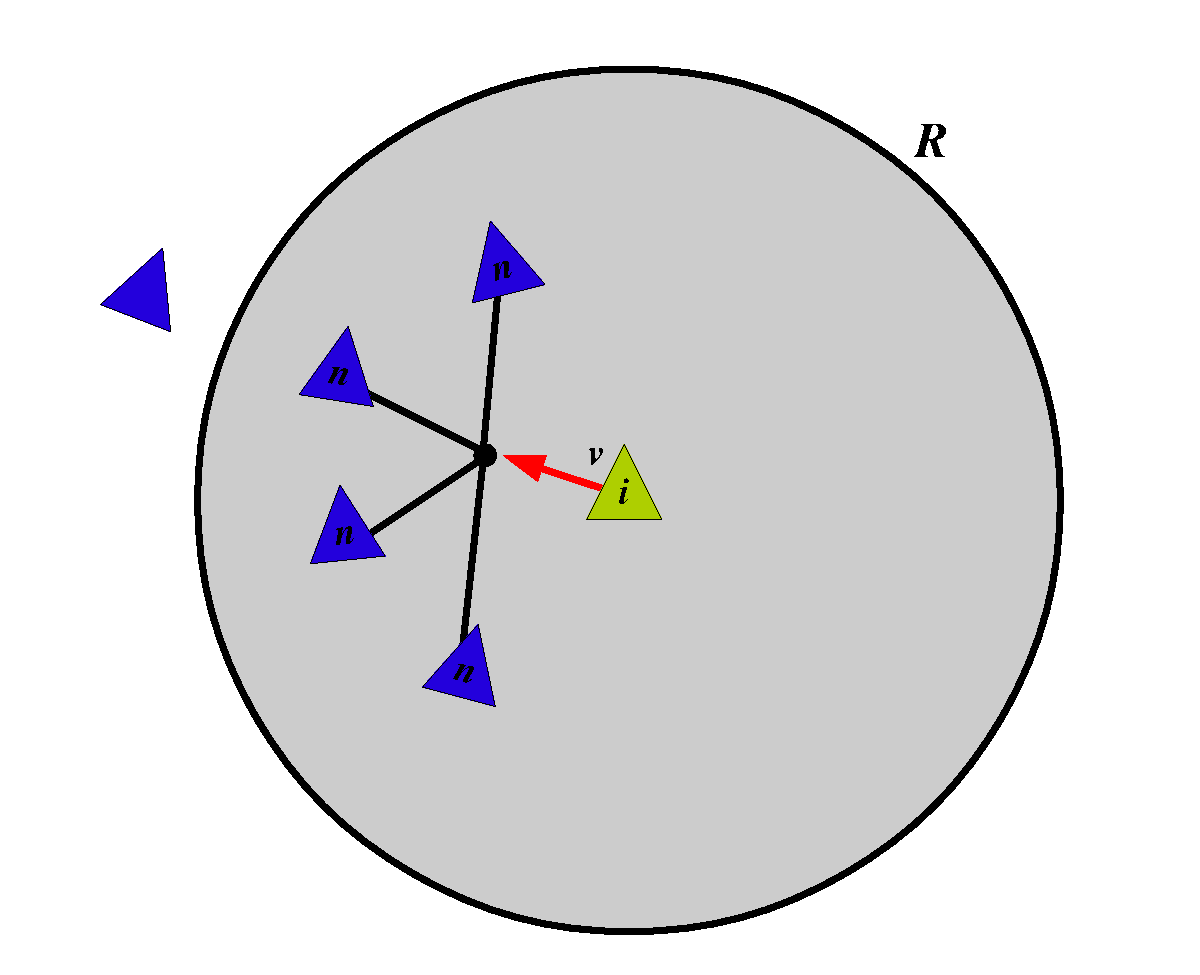
\includegraphics[scale=0.3]{figures/cohesion.pdf}
\caption{Cohesion steering force}
\label{cohesionPDF}
\end{center}
\end{figure}

The formula that we used for \textit{cohesion} is very similar to the formula used for \textit{alignment}, the only difference is that \textit{cohesion} uses the positions of the boid and \textit{alignment} uses the velocities. Equation~\ref{cohesionEquation} shows the \textit{cohesion} formula.

% cohesion equation
\begin{equation}
\label{cohesionEquation}
Cohesion = \left[  \frac{1}{N} \sum_{n=1}^{N} p_n \right ] - p_i
\end{equation}

Where $N$ is the number of boids in the local neighborhood of boid $i$. $p_n$ is the position of flockmate $n$. We average the position of the local flockmates in order to get the average position of the local neighborhood of boid $i$. Then, we subtract the current boid $i$ from the average position. That would give us the \textit{cohesion} force vector.

% other behaviors
\section{Other Steering Behaviors}
Besides the three main steering behaviors discussed in the above section many more steering forces have been previosly developed, see Section~\ref{currentwork} for a list of some of them. In this section we are going to discuss only the behaviors we implemented: \textit{goal}, \textit{avoid}, and \textit{follow the leader}.

% goal
\subsection{Goal}
\textit{Goal} is the steering behavior that attracts the boids to a specific location in global space. This location is static. Figure~\ref{seekfleePDF} shows the action taken when we want to approach or avoid the target. The red vector shows the \textit{goal} steering, the blue vector, avoid, which is discussed in the next section. The gray vector to the right of the boid is the desired velocity and the dotted line would be the path taken by the boid.

% seek and flee figure
\begin{figure}[htbp]
\begin{center}
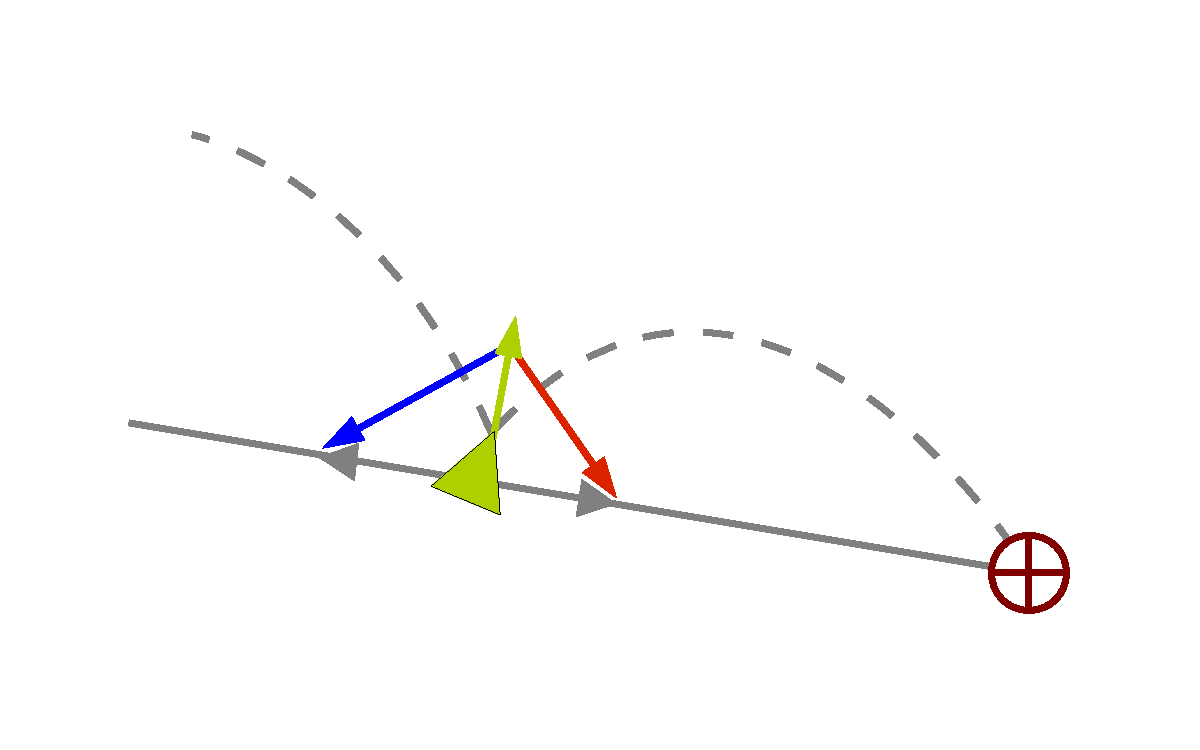
\includegraphics[scale=0.5]{figures/seekANDflee.pdf}
\caption{Goal and Avoid behaviors}
\label{seekfleePDF}
\end{center}
\end{figure}

\textit{Goal} behavior adjusts the boid's velocity in a way that it is aligned towards the target. So, \textit{how do we compute it?} Since the target is static, we subtract the position of the boid and the position of the target, normalized and multiply it by the current speed of the boid. This would gave us the desired velocity at what we would like to steer. Then, to get the steering vector, we subtract the current velocity from the desired velocity. The formula is in equation~\ref{goalEquation}

% goal equation
\begin{equation}
\label{goalEquation}
Goal = ((p_i - p_t) * v_i) - v_i
\end{equation}

Where $p_i$ and $v_i$ are the position and velocity of boid $i$, respectively. This rule will cause that the boid will keep approaching the goal over and over, kind of like moth buzzing around a light bulb.

% avoid
\subsection{Avoid}
\textit{Avoid} means to steer away from a static target in the global space. The approach is similar to the one taken for \textit{goal} with the difference that the desired velocity will be pointing to the opposite direction. Figure~\ref{seekfleePDF} depicts the steering vector in blue and the desired velocity in gray (at the left side of the boid). Notice that the desire velocity vector for both \textit{goal} and \textit{avoid} are pointing in opposite directions. Equation~\ref{avoidEquation} shows the mathematical formula for \textit{avoid}.

% avoid equation
\begin{equation}
\label{avoidEquation}
Avoid = -((p_i - p_t) * v_i) - v_i
\end{equation}

We called $((p_i - p_t) * v_i)$ the desired velocity, and here it has a negative sign preceding it, so that means that it is going to point in the opposite direction than the desired velocity of ~\textit{goal}.

% leader following
\subsection{Follow the Leader}
\textit{Follow the Leader} is the behavior in which there is a boid in charge of the flock, called \textit{leader}, and the boids that follow it are the \textit{followers}. This is one of the many complex behaviors that a flock can exhibit. There is a pattern, individual boids evaluate different rules. Followers would act like a point slightly behind the leader is its target, while the leader would approach randomly selected locations as its target.

% leader following figure
\begin{figure}[htbp]
\begin{center}
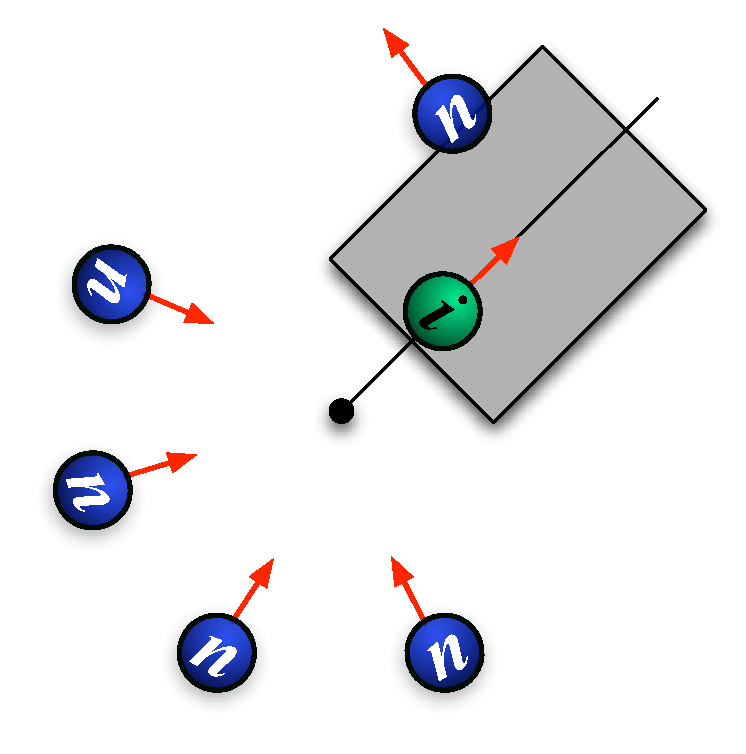
\includegraphics[scale=0.5]{figures/leaderFollowing.pdf}
\caption{Leader Following behavior}
\label{leaderPDF}
\end{center}
\end{figure}

Most of the time the followers want to stay closer to the leader without getting into its way. As can be seen in Figure~\ref{leaderPDF}.  If the follower is inside the rectangular region in front of the leader it would move away from it, leaving the way for the leader to move free without worrying of colliding with flockmates. The leader would compute its movement using equation~\ref{goalEquation} where $p_t$ is a random position within the global space. The followers that are outside the rectangular region will approach a point slightly behind from the leader using equation~\ref{goalEquation}.

% combining behaviors
\section{Combining the Steering Behaviors}
Each of the steering behaviors discussed above would return a velocity vector. Now the question is \textit{how do we combine it in order to move the boid?}. First, each steering force is normalized, then we weight them\footnote{Weights are given by the user, they are not constant values set it by us.}. For example, if we would like to combine \textit{separation}, \textit{alignment}, and \textit{cohesion} only, we would use equation~\ref{combine}. Each behavior is multiplied by a constant, then we add them up to get the acceleration vector.

% combine equation
\begin{equation}
\label{combine}
acceleration = Separation * C_S + Alignment * C_A + Cohesion * C_C
\end{equation}

Now that we have the acceleration, we add this acceleration to the current velocity to obtain the new velocity and we do \textit{Euler's Integration} to obtain the new position. See equation~\ref{velocity}, where $v_i$ and $p_i$ are the velocity and position of of boid $i$, respectively, and equation~\ref{integrate} where $dt$ is the time step. 

% integrate equation
\begin{align}
\label{velocity}
v_i = v_i + acceleration\\
\label{integrate}
p_i = p_i + dt * v_i
\end{align}

By doing this we finally obtain a new position for each of the boids. Recalling that each of these rules are going to be calculated for each boid every time step. \textcolor{red}{** OLMO: explain more this last part **}

% algorithm
\section{Algorithm}
\textcolor{red}{TODO: Write the algorithm in pseudocode}
